\documentclass[12pt, a4paper]{article}
\usepackage[a4paper, left=2cm, right=2cm, top=3cm, bottom=3cm]{geometry}

\usepackage[english]{babel}
\usepackage[utf8]{inputenc}
\usepackage{fancyhdr}

\usepackage{enumitem}
\usepackage{amsmath}
\usepackage{mathtools}
\usepackage{listings}

\usepackage{tikz}
\usetikzlibrary{arrows.meta,shapes.multipart}

\pagestyle{fancy}
\fancyhf{}
\lhead{Tutorium 02 \\ Abgabegruppe 01}
\chead{Blatt 04 \\ DatKom}
\rhead{Andrés Montoya, 405409 \\ Til Mohr, 405959}

\begin{document}

\begin{center}\fcolorbox{red}{yellow}{\begin{minipage}{35em}
	Bei uns war ursprünglich noch ein Dritter in unserer Abgabegruppe eingeteilt. Wir haben ihn vor über einer Woche versucht per E-Mail zu erreichen, leider erfolglos.\\
	Nach Ablauf der Anmeldefrist zu den Abgabegruppen haben wir gesehen, dass diese Person leider unsere Abgabegruppe verlassen hat.\\
	Bisher konnten wir noch keinen Dritten für unsere Abgabegruppe finden.\\
	Uns wurde auch seit dem letzten Blatt keine weitere Person zugeteilt.
\end{minipage}}\end{center}



\section*{Aufgabe 4.1}
\begin{enumerate}[label=\alph*)]
	\item	Maximale Rahmengröße: $$12 \text{B} + 1600 \text{B} \hat{=} 96 \text{b} + 12800 \text{b} = 12896 \text{b}$$
			Übertragung eines Rahmens: $$\frac{4}{1000} \text{s} + \frac{12896 \text{b}}{100 \cdot 10^6 \frac{\text{b}}{\text{s}}} = 0.00412896 \text{s}$$
			Übertragung eines ACK: $$\frac{4}{1000} \text{s} + \frac{96 \text{b}}{100 \cdot 10^6 \frac{\text{b}}{\text{s}}} = 0.00400096 \text{s}$$
			Maximale Nutzdatenrate: $$\frac{12800 \text{b}}{0.00412896 \text{s} + 0.00400096 \text{s}} = 1574431.23672 \frac{\text{b}}{\text{s}} \hat{=} 1.57443123672 \frac{\text{Mb}}{\text{s}}$$
	\item	Wahrscheinlichkeit, dass eine komplette Übertragung (Rahmen + ACK) erfolgreich ist: $$(1 - 10^{-4})^{12896 \text{b} + 96 \text{b}} = 0.272732187262$$
			Mittlere Nutzdatenrate: $$0.272732187262 \cdot 1574431.23672 \frac{\text{b}}{\text{s}} = 429398.074885 \frac{\text{b}}{\text{s}} \hat{=} 429.398074885 \frac{\text{kb}}{\text{s}}$$
	\item	\begin{enumerate}[label=\roman*)]
				\item	Um die Ntzdatenrate aus a) zu erreichen, können wir die Rahmengröße auf $1$ setzen. Dadurch arbeitet unser Sliding-Window-Verfahren genauso wie das Stop-And-Wait-Protokoll, weshalb die Nutzdatenrate gleich ist.
				\item	Es dauert mindestens $$0.00412896 \text{s} + 0.00400096 \text{s} = 0.00812992 \text{s}$$, bis der erste Rahmen des Fensters bestätigt wird.\\
						Das Absenden eines Rahmens beträgt $$\frac{12896 \text{b}}{100 \cdot 10^6 \frac{\text{b}}{\text{s}}} = 0.00012896 \text{s}$$
						Um die Leistung des Kanals komplett ausnutzen zu können, müssen wir mindestens so viele Rahmen in unserer Fensterzeit $0.00812992 \text{s}$ senden, dass keine Pausen entstehen. Damit benötigen wir eine Fenstergröße von mindestens 
						$$\lceil \frac{0.00812992 \text{s}}{0.00012896 \text{s}} \rceil = \lceil 63.0421836228 \rceil = 64$$
						Rahmen.\\
						Ab unter 64 Rahmen pro Fenster, sprich z.B. 63 Rahmen, hätten wir schon eine Wartezeit von mindestens $0.00000544 \text{s}$. In dieser Zeit ist der Kanal ungenutzt.
			\end{enumerate}
\end{enumerate}


\newpage


\section*{Aufgabe 4.2}
\begin{enumerate}[label=\alph*)]
	\item	\begin{enumerate}[label=\roman*)]
				\item	Latenz: $$\frac{1000 \text{km}}{200000 \frac{\text{km}}{\text{s}}} = \frac{1}{200} \text{s}$$
						Senden eines Rahmens: $$\frac{2500 \cdot 8 \text{b}}{1 \cdot 10^9 \frac{b}{s}} = 0.00002 \text{s}$$
						Es kann also ein Rahmen alle $0.00002 \text{s}$ auf die Leitung gelegt werden. Es braucht nun weitere $(\frac{1}{200} \text{s} + 0.00002 \text{s}) + \frac{1}{200} \text{s} = 0.01002 \text{s}$ bis die Bestätigung des Rahmens ankommt.\\
						Anzahl Rahmen: $$\frac{0.01002 \text{s}}{0.00002 \text{s}} = 501$$
				\item	Da wir $501$ Rahmen "gleichzeitig" senden können, benötigen wir mind. $501 + 1$ Sequenznummern. Diese können wir mit $9$ Bit darstellen: $$\lceil lb(502) \rceil = 9$$
				\item	Es gibt keinen Unterschied in der Rahmengröße hier. Aus diesem Grund kann man wie bei der ii) $9$ Bit für die Darstellung der Sequenznummern verwenden.
			\end{enumerate}
	\item	$$\frac{501 \cdot 2450 \cdot 8 \text{b}}{0.01002 \text{s}} = 980000000 \frac{\text{b}}{\text{s}} \hat{=} 980 \frac{\text{Mb}}{\text{s}}$$
\end{enumerate}


\newpage


\section*{Aufgabe 4.3}
\begin{enumerate}[label=\arabic*.]
	\item	Da alle Weiterleitungstabellen leer sind, broadcastet jeder Switch (und jeder Hub sowieso) den ersten Rahmen. Damit bekommen auch alle Rechner (außer A, Switch 1 boradcastet nicht an Port 1.1, da der Rahmen von dort kam) diesen Rahmen.\\
			
			Switch 1:
			\begin{center}
				\begin{tabular}{c|c}
					1.1 & A \\
					\hline
					1.2 \\
					\hline
					1.3 \\
					\hline
					1.4 \\
				\end{tabular}
			\end{center}
			
			Switch 2:
			\begin{center}
				\begin{tabular}{c|c}
					3.1 & A \\
					\hline
					3.2 \\
					\hline
					3.3 \\
				\end{tabular}
			\end{center}
			
			Switch 3:
			\begin{center}
				\begin{tabular}{c|c}
					4.1 & A \\
					\hline
					4.2 \\
					\hline
					4.3 \\
				\end{tabular}
			\end{center}
			
			Switch 4:
			\begin{center}
				\begin{tabular}{c|c}
					6.1 & A \\
					\hline
					6.2 \\
				\end{tabular}
			\end{center}
	
	\item	C sendet nun über 2.2 einen Rahmen nach A an Hub 1. Hub 1 broadcastet den Rahmen an Switch 1 und Switch 2. Weder Switch 1 kennt den Port von A (1.1) und sendet ihm diesen. Switch 2 kennt auch den Port von A, jedoch liegt er an 3.1, also an dem Port, an dem er den Rahmen erhalten hat. Switch 2 dropped also den Rahmen.\\
	
			Switch 1:
			\begin{center}
				\begin{tabular}{c|c}
					1.1 & A \\
					\hline
					1.2 \\
					\hline
					1.3 & C \\
					\hline
					1.4 \\
				\end{tabular}
			\end{center}
			
			Switch 2:
			\begin{center}
				\begin{tabular}{c|c c}
					3.1 & A & C \\
					\hline
					3.2 \\
					\hline
					3.3 \\
				\end{tabular}
			\end{center}
			
			Switch 3:
			\begin{center}
				\begin{tabular}{c|c}
					4.1 & A \\
					\hline
					4.2 \\
					\hline
					4.3 \\
				\end{tabular}
			\end{center}
			
			Switch 4:
			\begin{center}
				\begin{tabular}{c|c}
					6.1 & A \\
					\hline
					6.2 \\
				\end{tabular}
			\end{center}
	
	\item	G sendet nun über 6.2 einen Rahmen nach A an Switch 4. Switch 4 weiß, dass A an Port 6.1 anliegt, also gibt er Switch 2 den Rahmen weiter. Switch 2 weiß, dass A an 3.1 anliegt, also gibt er den Rahmen an Hub 1 weiter. Hub 1 broadcastet nun das Signal an Rechner C und Switch 1. Switch 1 weiß, dass A an 1.1 anliegt.
			
			Switch 1:
			\begin{center}
				\begin{tabular}{c|c c}
					1.1 & A \\
					\hline
					1.2 \\
					\hline
					1.3 & C & G \\
					\hline
					1.4 \\
				\end{tabular}
			\end{center}
			
			Switch 2:
			\begin{center}
				\begin{tabular}{c|c c}
					3.1 & A & C \\
					\hline
					3.2 \\
					\hline
					3.3 & G\\
				\end{tabular}
			\end{center}
			
			Switch 3:
			\begin{center}
				\begin{tabular}{c|c}
					4.1 & A \\
					\hline
					4.2 \\
					\hline
					4.3 \\
				\end{tabular}
			\end{center}
			
			Switch 4:
			\begin{center}
				\begin{tabular}{c|c}
					6.1 & A \\
					\hline
					6.2 & G\\
				\end{tabular}
			\end{center}
\end{enumerate}


\newpage


\section*{Aufgabe 4.2}
\begin{enumerate}[label=\alph*)]
	\item	Man könnte einen solchen Switch immer als root bridge wählen, indem man ihm die niedrigste ID gibt (zB 0), und dann als root bridge immer den Switch mit der geringsten ID wählt.\\
			Es ist sinnvoll einen solchen Switch als root bridge zu wählen, wenn ein hoher Anteil an Kommunikation mit dem Internet stattfindet. Denn dann ist der ST so aufgebaut, dass alle Switches einen möglichst schnellen Weg (minimale Kosten) zur root bridge haben. Damit kann also die Datenrate im Netzwerk erhöht werden.
	\item	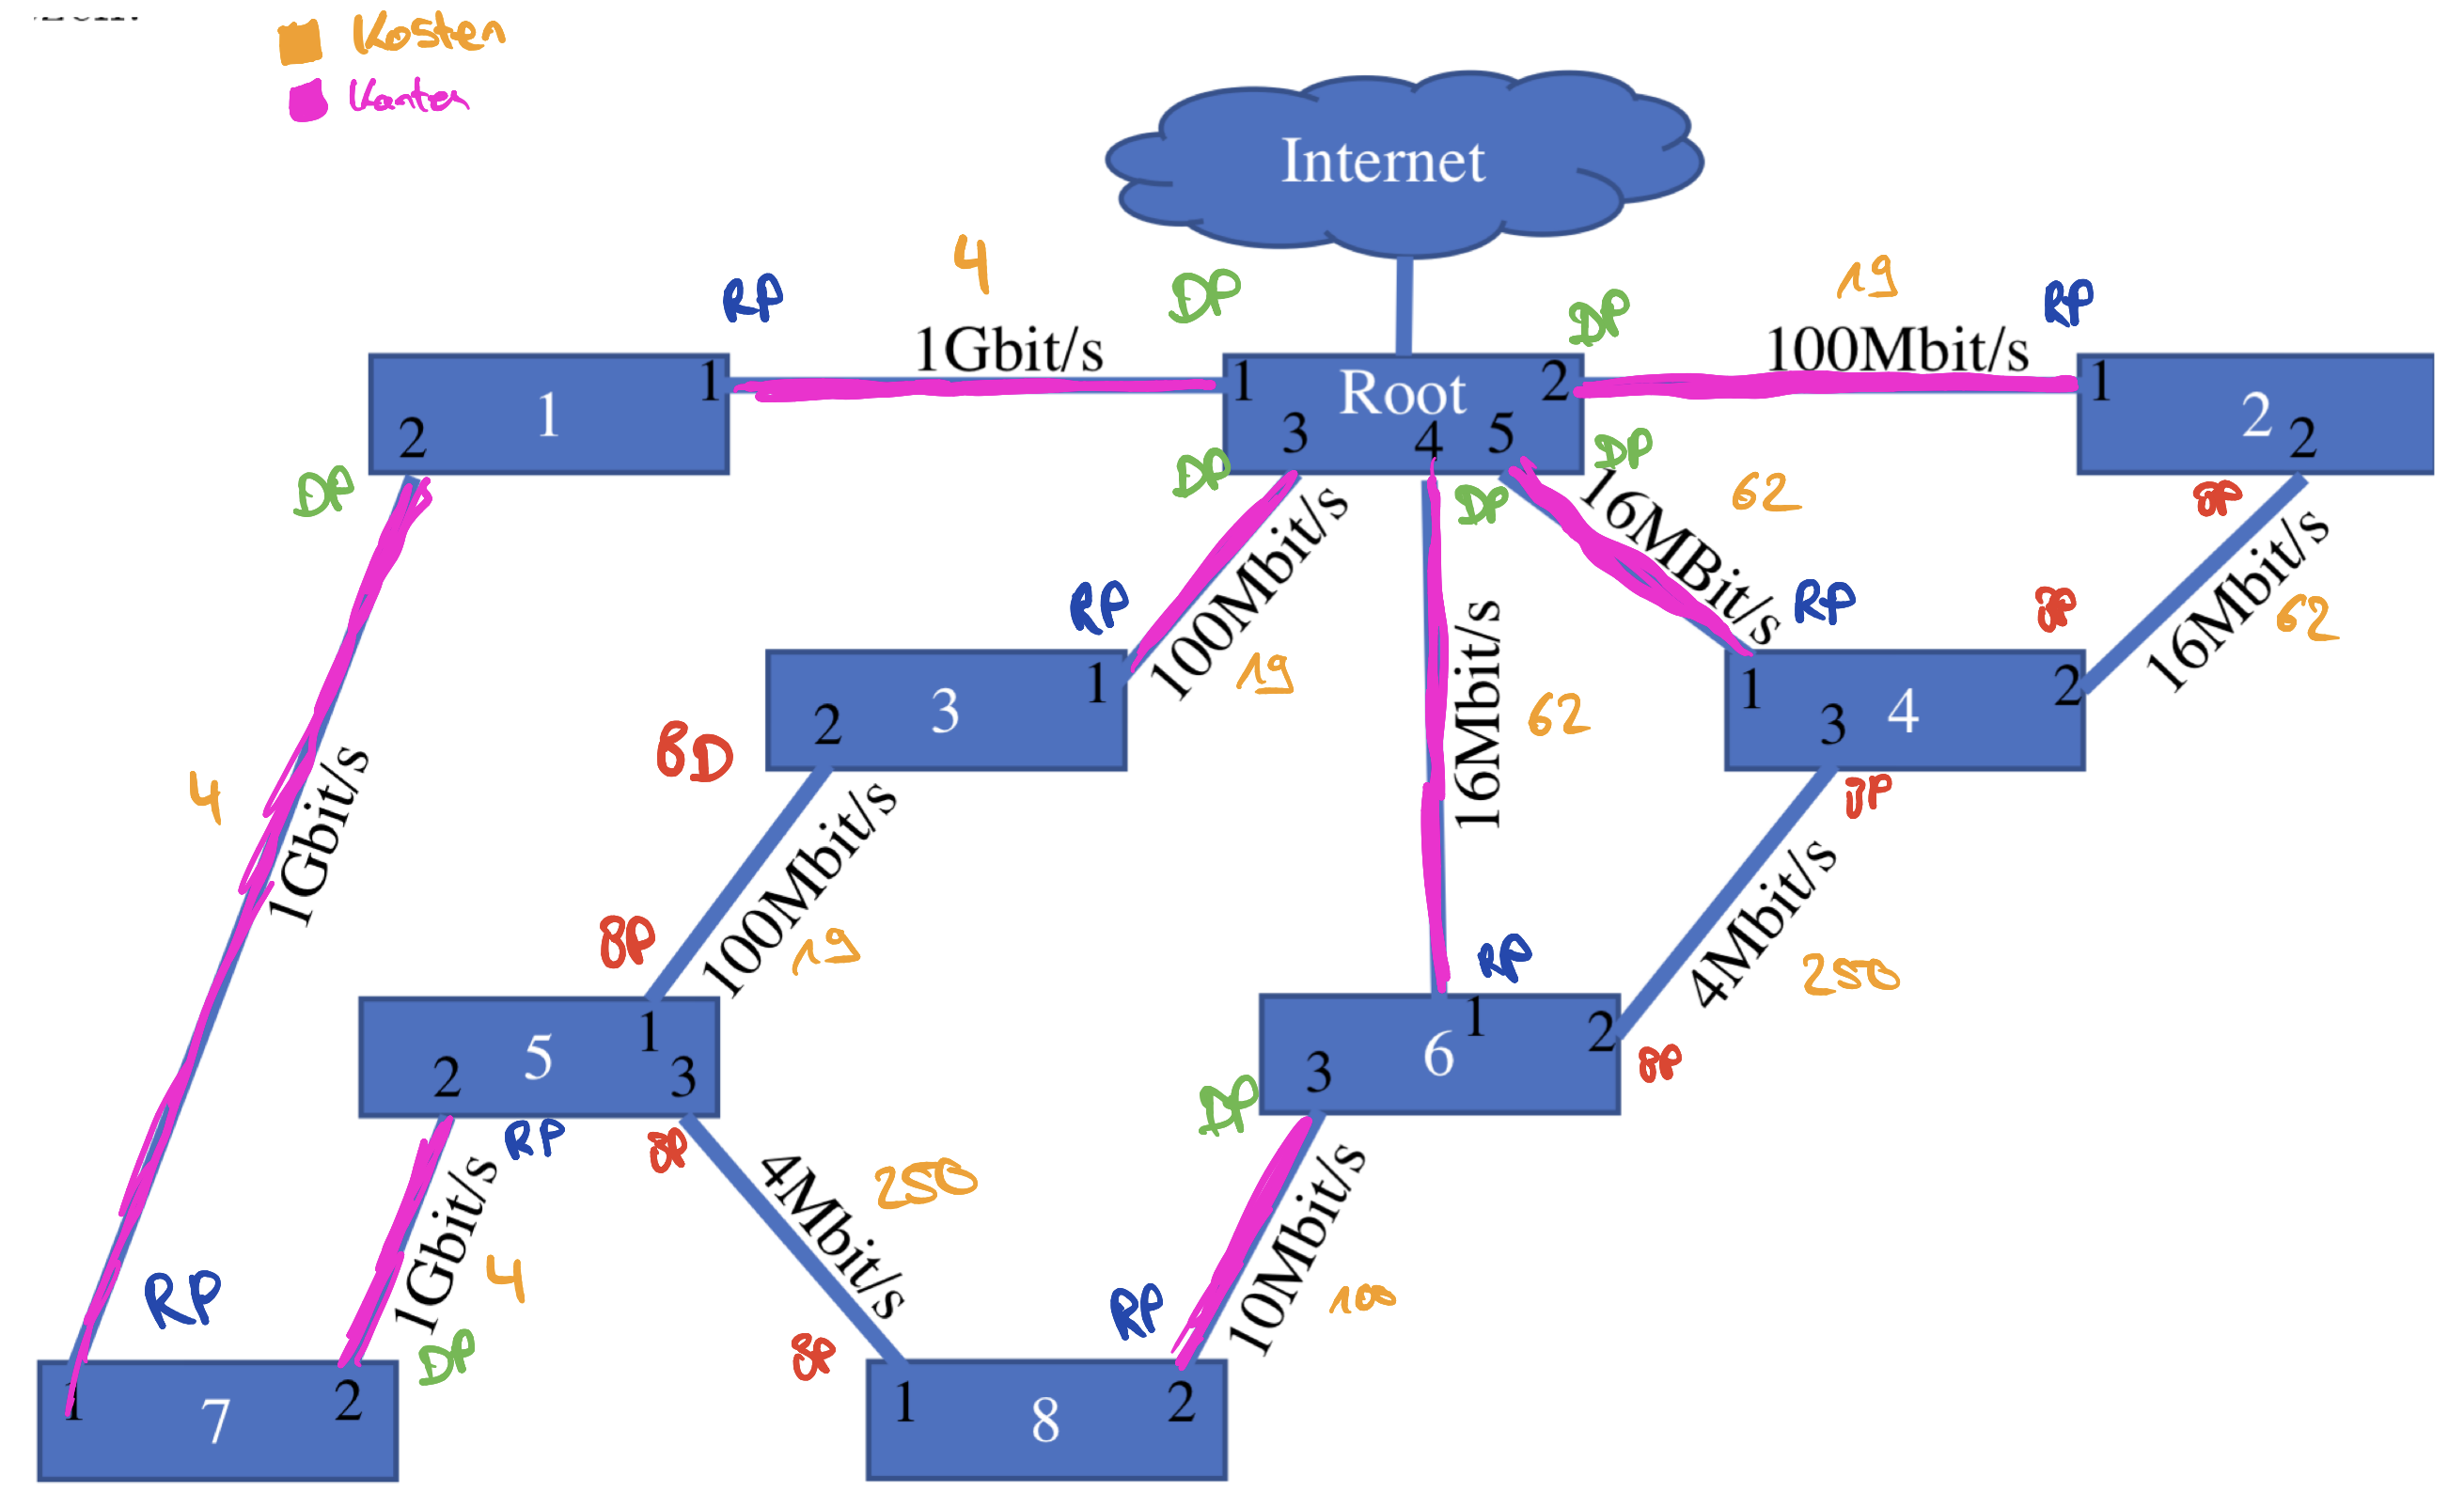
\includegraphics[scale=0.36]{4.4_b.png}
\end{enumerate}

\end{document}